\documentclass{cslthse-msc}
\usepackage[utf8]{inputenc}
\usepackage[english]{babel}
\usepackage{amsmath}
\usepackage{amsfonts}
\usepackage{amssymb}
\usepackage{amsthm}
%\usepackage{makeidx}
\usepackage{graphicx}
\usepackage[titletoc, header, page]{appendix}

\usepackage{hyperref}
\usepackage{pdfpages}
\usepackage{rotating}
\usepackage{enumitem}
\usepackage{subfig}
\usepackage{float}
\usepackage{listings}
\usepackage{epstopdf}
%% listings-modelica.cfg
%% Copyright 2014 Martin Sjoelund, Dietmar Winkler
%
% This work may be distributed and/or modified under the
% conditions of the LaTeX Project Public License, either version 1.3
% of this license or (at your option) any later version.
% The latest version of this license is in
%   http://www.latex-project.org/lppl.txt
% and version 1.3 or later is part of all distributions of LaTeX
% version 2005/12/01 or later.
%
% This work has the LPPL maintenance status `maintained'.
%
% The Current Maintainer of this work is Dietmar Winkler
%
% Code repository https://github.com/modelica-tools/listings-modelica
%
% This work consists of the file listings-modelica.cfg

\lstdefinelanguage{modelica}
{
  morekeywords=[1]{
    algorithm,and,annotation,as,assert,block,break,case,class,connect,connector,
    constant,constrainedby,der,discrete,each,else,elseif,elsewhen,encapsulated,
    end,enumeration,equality,equation,expandable,extends,external,failure,final,
    flow,for,function,guard,if,import,in,initial,inner,input,List,local,loop,
    match,matchcontinue,model,not,operator,Option,or,outer,output,package,parameter,
    partial,protected,public,record,redeclare,replaceable,return,stream,
    subtypeof,then,Tuple,type,uniontype,when,while},
  morekeywords=[2]{true, false},
  % Do not make true,false keywords because fn(true,x, false ) shows up as fn(true,x, *false*)
  sensitive=true,
  comment=[l]//,
  morecomment=[s]{/*}{*/},
  alsodigit={.,-},
  morestring=[b]',
  morestring=[b]",
}[keywords,comments,strings]

\definecolor{keywordcolor1}{rgb}{0,0,.4}
\definecolor{keywordcolor2}{rgb}{.90,0,0}
\definecolor{stringcolor}{rgb}{0.133,0.545,0.133}
% \definecolor{listingbgcolor}{rgb}{0.95,0.95,0.95}

\lstset{
  breaklines=true,
  language=modelica,
  basicstyle=\ttfamily,
  keywordstyle=[1]\color{keywordcolor1}\bfseries,
  keywordstyle=[2]\color{keywordcolor2},
  stringstyle=\color{stringcolor},
%  backgroundcolor=\color{listingbgcolor},
  framexleftmargin=5pt,
  xleftmargin=5pt,
  xrightmargin=5pt,
  showstringspaces=false
}

\newcommand{\code}[1]{\lstinline|#1|}
\newcommand{\modelica}[1]{\lstinline[language=modelica]|#1|}


%\geometry{showframe}

\author{
	Erik Hedblom \\
	{\normalsize \href{mailto:hedblom.e@gmail.com}{\texttt{hedblom.e@gmail.com}}}
	\and
	Kasper Rundquist \\
	{\normalsize \href{mailto:kasper.rundquist@gmail.com}{\texttt{kasper.rundquist@gmail.com}}}
}

\title{Safe test selection for Modelica using static analysis}
%\subtitle{A {\LaTeX} class}
\company{Modelon AB}
\supervisors{Johan Ylikiiskilä, \href{mailto:johan.ylikiiskila@modelon.com}{\texttt{johan.ylikiiskila@modelon.com}}}{Jonatan Kämpe, \href{mailto:jonathan.kampe@modelon.com}{\texttt{jonathan.kampe@modelon.com}}}{Niklas Fors, \href{mailto:niklas.fors@cs.lth.se}{\texttt{niklas.fors@cs.lth.se}}}%\supervisor{Niklas Fors, \href{mailto:niklas.fors@cs.lth.se}{\texttt{niklas.fors@cs.lth.se}}}
\examiner{Görel Hedin, \href{mailto:gorel.hedin@cs.lth.se}{\texttt{gorel.hedin@cs.lth.se}}}

\date{\today}
%\date{January 16, 2015}

\acknowledgements{
%TODO: Write acknowledgements

%%If you want to thank people, do it here, on a separate right-hand page. Both the U.S. \textit{acknowledgments} and the British \textit{acknowledgements} spellings are acceptable.
}

\theabstract{
During software development testing of the software can be very time consuming. We have developed a safe regression test selection for the programming language Modelica. By excluding tests that not will detect any errors it is possible to reduce the testing time, since Modelica tests takes very long time to run there is much time to save. As far as  we know this has previously not been done for Modelica. To do the test selection we have implemented a dependency analysis of Modelica classes in an existing Modelica compiler. When we look at the commit history of the Modelica Standard Library and compare running all tests with only running the tests selected by our test selection, the timed saved for running tests is in this case 56\% of the time it takes to run all tests.
%TODO: Update the abstract when we have done a version of the test selection not limited by the lookup in the source tree in OCT.

%%Your abstract should capture the whole thesis with focus on the problem and solution in 150 words. Avoid acronyms, footnotes, and references in the abstract if possible.

}

% TODO: Provide a few keywords relevant for your report. Use five to six words, of which at most two should be from the title.
\keywords{Test Selection, Modelica, JastAdd, Regression testing}

\divisionoflabor{
}

%% Only used to display font sizes
\makeatletter
\newcommand\thefontsize[1]{{#1 \f@size pt\par}}
\makeatother
%%%%%%%%%%


\begin{document}
\makefrontmatter
\chapter[Introduction]{Introduction}

\section{Motivation}
Software tests are used to verify that software works as intended.
During software development, when a change is integrated into a project all previous testing have to be rerun. \cite{DBLP:conf/sigsoft/LegunsenHSLZM16, haider2016safe} This is know as regression testing. Test suites usually accumulates over time and regression testing can therefore be very time consuming. Depending on the change some or most of the tests may be unrelated to the change and therefore unnecessary to run. By excluding unrelated tests significant time savings could be achieved. This is called test selection and have to our knowledge not been previously done for Modelica. Modelica is a high level programming language used for simulations in various areas. In Figure \ref{fig:bouncingBallCode} is an example of Modelica code, it shows a model of a bouncing ball and a model with two instances of a bouncing ball. When the test selection is done for regression tests it is known as regression test selection (RTS). 

\begin{figure}[!htbp]
    \centering
    {\lstinputlisting[language=modelica]{Modelica/BouncingBall.mo}}
    \caption{Modelica example bouncing ball, retrieved from \cite{aakesson2010implementation}}.
    \label{fig:bouncingBallCode}
\end{figure}

\section{Goal}
The aim of this project is to reduce testing times for Modelica projects without loss of quality. This will be done by developing and implementing a safe RTS method, a method to exclude tests in a test suite unaffected by a specific change. \cite{DBLP:conf/pppj/OqvistHM16} Regression testing can then be performed with a reduced test suite without compromising testing quality.

\section{Results}
We have succeeded in decreasing the time for testing by test selection for Modelica. In chapter 5 we try to assess, how much time can be saved with our RTS method and the precision of the method. We look at the commit history for some Modelica libraries to see how much time would have been saved if our RTS method had been used instead of running all tests for each commit. However we cannot prove that the method we have developed is safe, we discuss this further in chapter 7.

\chapter[Background]{Background}
\section{Test Selection}
A safe Regression Test Selection (RTS) method will select at least all tests that produce a new result after a specific change. \cite{DBLP:conf/pppj/OqvistHM16} A safe RTS method is therefore equivalent, in quality, to running all tests. For a RTS method to be useful the RTS algorithm should run in less time than it takes to run the excluded tests. This is not necessary for each run, but on average the overhead needs to be less than the time it takes to run the excluded tests.

Precision is a measurement of how good the test selection is. \cite{DBLP:conf/sigsoft/LegunsenHSLZM16} If fewer redundant tests are selected the test selection has higher precision. There is a trade-off between the precision of the test selection and the overhead. If a RTS algorithm has full precision it doesn't select any tests that can't fail. But the higher precision the more complex algorithm is needed. For a more complex algorithm its harder to follow the rules and verify that the RTS method is safe. A more complex algorithm also creates more overhead.

\section{Modelica}
Modelica is a declarative, object oriented programming language where models are described by equations. It is used to perform high performance simulations. This section will introduce the parts of Modelica important for this project.

Modelica uses dot notation like many other languages to access something inside an object. Consider the code snippet in Figure \ref{fig:modelicaExample}, Model \texttt{M} can be accessed though \texttt{P1.P2.M}. We will call this an access. Depending on from which scope \texttt{M} is being accessed the access could also be \texttt{P2.M} or just \texttt{M}. An access using dot notation is basically a list of accesses and we will call all the accesses before the last access, the path. For instance, \texttt{P1.P2} is the path of \texttt{P1.P2.M}. We will also denote an access, where the first part of it is referencing the top package in the library, as a qualified name.

\begin{figure}[!htbp]
    \centering
    \subfloat{{\includegraphics[scale=0.8]{dotGenerated/ModelicaExample.eps}}}
    \qquad
    \subfloat{\raisebox{3.2 cm}{\lstinputlisting[language=modelica]{Modelica/ModelicaExample.mo}}}
    \caption{Example of Modelica structure}
    \label{fig:modelicaExample}
\end{figure}

It is not apparent from an access what it is trying to access, it could be a package, model, function or a component. Due to this we will simplify the terminology by grouping models, packages and function together and just call them classes. Components are instantiations of models and will be handled separately since our solution can not resolve accesses to components yet.

\subsection{Name lookup}
In order to find a match for a name, Modelica starts by looking at the first name in a qualified name. Take for example the qualified name Modelica.Fluid.Pipes.StaticPipe. In this example Modelica is the first name in the qualified name.
\begin{itemize}
\item To find a match for the name, Modelica first checks if it's a built in type. If it's a built in type Modelica has found a match for the name.

\item If it's not a built in type Modelica looks in the class where the name is used, including inherited definitions, for a nested definition of the name. 

\item If there is no nested definition of the name, Modelica looks in the imports in the class where the name is used, inherited imports are not included, to find a match for the name.

\item If a match for the name is not found in the imports, Modelica looks for a nested definition in the enclosing package, including inherited definitions.

\item If the definition of the name is not found in the enclosing package, Modelica looks for a imported definition, not including inherited imports, in the enclosing package.
\end{itemize}
If a match for the name still not is found, Modelica continues by using the same method and looking in the enclosing packages enclosing package and so on until: the enclosing package has the encapsulated qualifier or a package is a root package, in which case it doesn't have an enclosing package. In the first case the search for the name terminates and in the second case Modelica searches for a match in root level packages.

The search is done in the same way for the first name in a qualified name and an unqualified name.

If a name is a part of a qualified name and is not the first name in the qualified name, it must be a nested definition within the definition of the previous name in the qualified name. In the example Modelica.Fluid.Pipes.StaticPipe, Fluid must be a nested definition within Modelica.\cite{modelicamodelica, tillermodelica}

\subsection{Import}
Imports are possible in Modelica to refer to a class or component in another package that is not in the same enclosing package. To find an imported object Modelica looks at root packages, so the qualified name needs to be used in an import. An import creates an alias. In the import below \texttt{HydralicConductance} will be mapped to the qualified name \texttt{Modelica.Fluid.Types.HydralicConductance}.

\lstinputlisting[language=modelica]{Modelica/import.mo}

Modelica offers the option to rename an import. Here an alias will be created where the name \texttt{Conductance} is mapped to the qualified name \texttt{Modelica.Fluid.Types.HydralicConductance}.

\lstinputlisting[language=modelica]{Modelica/renamedImport.mo}

Modelica allows the use of wildcard imports. Using wildcards it is not possible to rename the import. This wildcard import will create an alias for every definition in \texttt{Modelica.Fluid}.

\lstinputlisting[language=modelica]{Modelica/wildcardImport.mo}

\section{Compiler}
JModelica.org is an open source compiler that is developed and maintained by Modelon. Optimica Compiler Toolkit (OCT) is the commercial version of JModelica.org. Our solution will be developed in OCT but will not use any OCT specific functionality. 

The compilation of Modelica code is done in several steps, see Figure \ref{fig:compilerSteps}. \cite{aakesson2010implementation} In the first step name and type analysis of the source code is done, identifiers are bound to declarations etc. An AST (Abstract Syntax Tree) is built in form of a source tree.


%TODO: Why setep 2 and 3?
In step two a new AST in form of a instance tree is generated from the source tree. Each node in the instance tree has a reference to the corresponding declaration in the source tree. The instance tree consists of instances of models. The root is the model chosen by the user to be flattened.

In the third step the Modelica code is flattened, a flat model is generated from the instance tree. In this step class, component and inheritance structures are removed. This results in a model that only has a set of equations and a set of variables.

In the fourth step the equations are sorted and optimized.

In the last step C-code is generated.

\begin{figure}[!htbp]
    \centering
    {\includegraphics[scale=0.5]{dotGenerated/CompilerSteps.eps}}
    \caption{The steps in the compilation.}
    \label{fig:compilerSteps}
\end{figure}

\section{JastAdd}
JModelica.org is developed using the Meta compiler JastAdd. JastAdd is a system based on reference attribute grammars ~\cite{aakesson2010implementation}, for extensible implementation of compilers. An Abstract Syntax Tree (AST) is used to represent a program. Attribute Grammars is a method for declaratively defining computations on an AST. A node in an AST can have a synthesized attribute or an inherited attribute. An attribute is defined by an equation. A synthesized attribute is defined in the node, an inherited attribute is defined in an ancestor node. A JastAdd specification is used to create an object-oriented framework.

Collection attributes are defined by partial definitions in a number of arbitrary nodes. ~\cite{magnusson2007extending}. A node that have a partial definition of a collection attribute contributes to the value of the collection attribute. A collection attribute is usually a set where the empty set is the initial value of the collection attribute. The contributors, the nodes that contributes to the collection attribute, can for example contribute by adding elements to the set.

\section{Model Testing Toolkit}
Model testing Toolkit (MTT) is a toolbox developed by Modelon to handle testing of Modelica projects. It has both a command line and a graphical interface and we will add functionality and options to both to support test selection.

\subsection{Tests}
    Write about runconfigs?

\chapter[Dependency analysis]{Dependency analysis}
To build the dependency graph we have constructed a set of rules to determine what creates dependencies. Due to limitations in JModelica.org, mainly pertaining to the lookup of names in the source tree, the rules have been adjusted to work around these limitations. When the look of an access fails in the source tree we say the access is not resolvable. This means that an valid access can still fail to resolve. We hope to have time to fix the limitations to perform a better and more accurate dependency analysis. First we introduce the rules and then we will go on and explain and motivate each one.

\paragraph{Dependency Rules}
\begin{enumerate}
\item A class depends on all resolvable accesses within it.
\item A class depends on its encapsulating class. 
\item All resolvable accesses in the path of an access yields dependencies.
\item A class depends on all classes encapsulated by the accessed class. If the access is not resolvable, the last resolvable access in the path will be used instead.
\item Exception to Rule 4: Rule 4 is not applicable to import statements. An import should not add dependencies to classes not imported but the import.
\end{enumerate}


\begin{figure}[!htbp]
    \centering
    \subfloat{{\includegraphics[scale=0.8]{dotGenerated/Parent.eps}}}
    \qquad
    \subfloat{\raisebox{3.2 cm}{\lstinputlisting[language=modelica]{Modelica/Parent.mo}}}
    \caption{A class depends on its encapsulating class}
    \label{fig:parentGraph}
\end{figure}

The first rule is perhaps the most intuitive, if a class accesses another class there is also a dependency to that class. However, due to the limitations in JModelica.org not all accesses in a class can be followed and therefor not all dependencies from this rule can be created. We will later see how the other rules compensate for this. 

The next rule, Rule 2, will create a dependency from a class to its encapsulating class. An example can be found in Figure \ref{fig:parentGraph}. In the example there is a constant \texttt{k} defined in package \texttt{P}. If another constant with the same name were to be added in in model \texttt{M1} the reference to \texttt{k} in \texttt{M2} will change to refer to the new constant and shadow the k in \texttt{P}. Therefore we need a dependency from \texttt{M2} to \texttt{M1} to handle name shadowing.

In Figure \ref{fig:parentGraph} we also expect Rule 1 to create a dependency from \texttt{M2} to \texttt{P} due to \texttt{k} being located in \texttt{P}. However, the access \texttt{k} cannot be resolved by the JModelica.org compiler in the source tree and we will miss the dependency to \texttt{P}. In this case we can see that Rule 2 can compensate by adding an indirect dependency from \texttt{M2} to \texttt{P}. 
If the constant k in package \texttt{P} is changed it will affect model \texttt{M2}. Therefore we need a dependency from \texttt{M2} to \texttt{P}. With Rule number 1 we get dependencies from \texttt{M2} to \texttt{M1} and from \texttt{M1} to \texttt{P}. So we have an indirect dependency from \texttt{M2} to \texttt{P}.

\begin{figure}[!htbp]
    \centering
    \subfloat{{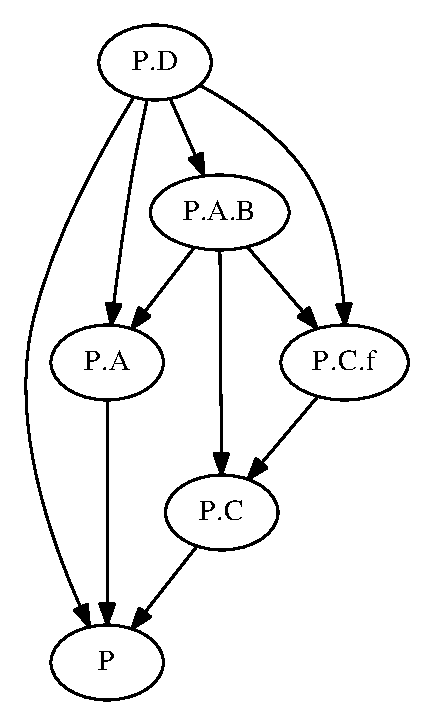
\includegraphics[scale=0.8]{dotGenerated/DotAccess.eps}}}
    \qquad
    \subfloat{\raisebox{9.5 cm}{
        \begin{minipage}[t]{.5\textwidth}
        \centering
        \lstinputlisting[language=modelica]{Modelica/DotAccess.mo}
        \end{minipage}}}
    \caption{Access with more access in its path, \texttt{P2.f}}
    \label{fig:dotAccess}
\end{figure}

In Figure \ref{fig:dotAccess}, we want dependencies from model \texttt{M} to all parts of the access to \texttt{f}. This means that in addition to a dependency to \texttt{f}, a dependency to \texttt{P3} is also required. If package \texttt{P3} is removed it will cause a compilation error when model \texttt{M} is compiled. Also, if \texttt{f} is shadowed in \texttt{P3} the behavior of model \texttt{M} will change. This is caught by Rule 3, that creates dependencies from \texttt{M} to \texttt{f} and \texttt{P3}.


\begin{figure}[!htbp]
    \centering
    \subfloat{{\includegraphics[scale=0.8]{dotGenerated/Component.eps}}}
    \qquad
    \subfloat{\raisebox{4.7 cm}{\lstinputlisting[language=modelica]{Modelica/Component.mo}}}
    \caption{Access through component}
    \label{fig:component}
\end{figure}

Rule 4 is needed to handle the case in Figure \ref{fig:component}. Ideally the access \texttt{m.M3.f} would create dependencies to \texttt{M2}, \texttt{M3} and \texttt{f}. Because \texttt{m} is a component and the analysis is done in the source tree, \texttt{P.M2.M3.f} cannot be resolved and no dependencies can be created. Instead Rule 4 is used to create dependencies to everything defined in \texttt{M3} when \texttt{m} is declared.
It is also possible that an access cannot be fully resolved. This is the case in \ref{fig:brokenAccess}, where the access \texttt{P1.m.f} cannot be resolved because the constant \texttt{m} is a component. In this case the only resolvable part is \texttt{P1} and a  dependency is created to \texttt{P1} by Rule 3. \texttt{P1} have dependencies to \texttt{M} and \texttt{f} through Rule 4. Hence, it is not a problem that Rule 4 cannot be applied to \texttt{P1.m.f}.

\begin{figure}[!htbp]
    \centering
    \subfloat{{\includegraphics[scale=0.8]{dotGenerated/BrokenAccess.eps}}}
    \qquad
    \subfloat{\raisebox{4.0 cm}{\lstinputlisting[language=modelica]{Modelica/BrokenAccess.mo}}}
    \caption{Access containing a component}
    \label{fig:brokenAccess}
\end{figure}

The exception to Rule 4 is added to improve the precision of the test selection. Imports are specific and it is enough to add dependencies to what is actually imported. It is not uncommon to import packages located high up in the library structure. Without this exception unnecessary dependencies would be added to all or large part of the library. For example in Modelica's standard library there are several imports of Modelica, which is the top level package. Such import would create dependencies to every single class in the library. (Such imports may seem unnecessary and in fact they often are, but they can be used to affect the name lookup if there exists classes with the same name in the library)  

\chapter[Implementation]{Implementation}
In this chapter we will describe how we have implemented the test selection. The solution is implemented both in OCT and MTT, where MTT will interact with the user and run the reduced test suit and OCT will produce the dependency graph.


\section{Model Testing Toolkit}

MTT will process the data from the user, either from the command line interface (CLI) or from the graphical user interface (GUI). We have have added an option to the CLI so the user can specify that test selection should be used and which models or files have changed. In the GUI we have added a menu option to specify which models have changed, this is shown in Figure \ref{fig:MTTrun}. In the GUI multiple models can be selected.

\begin{figure}[!hbtp]
    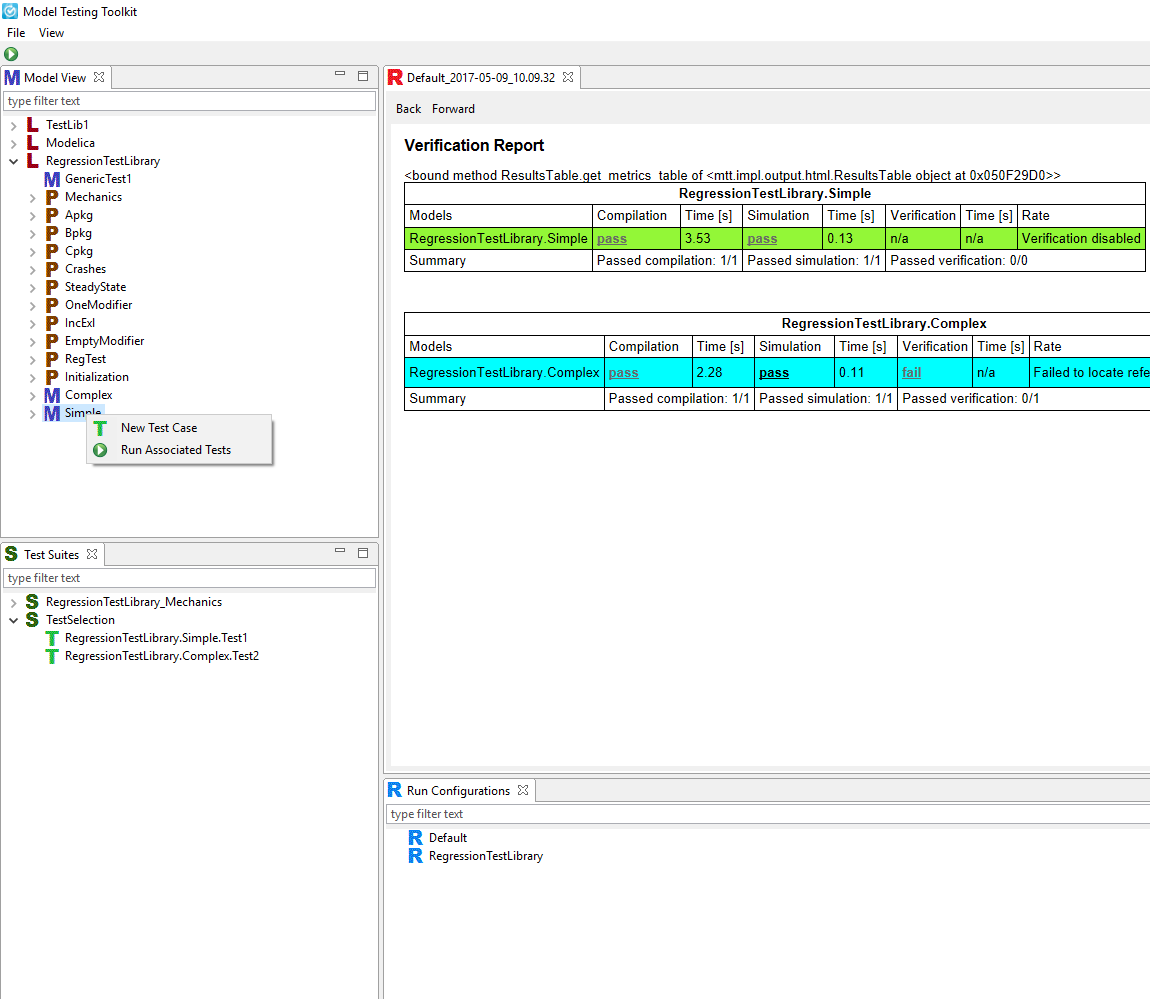
\includegraphics[width=1.0\textwidth]{Pictures/MTT_Capture.png}
    \caption{A screen shot of the MTT GUI}
    \label{fig:MTTrun}
\end{figure}

MTT will then send all modified files or models to OCT and ask for all affected models. Then all tests testing one of the affected models will be selected and run.

\subsection{Change detection}
There is no automatic change detection, instead the user manually have to specify which models or files should be considered changed. Automatic change detection could be implemented using a version control system such as Git or SVN. A build server could look at the commit history to determine what is changed and commands such as \texttt{git status} and \texttt{svn info} could be used when a user is using the tool. Another option is to look at the file timestamps to determine what is changes.

\section{Dependency analysis}
We have previously described how the dependency analysis should be performed. In this section we will look at some of the aspects not handles by the rules presented in Chapter 3.

\subsection{Scope}
To speed up the dependency analysis we ask the user to specify which libraries should be search for dependencies. For example, the standard library is automatically included in projects but users will rarely make changes to or test it. Hence, searching for dependencies to and in the standard library will usually be unnecessary. There might also be other dependencies in a project that are considered stable and unnecessary to analyze. In MTT this is handled by automatically search all open libraries.

Furthermore, our implementation also excludes Modelica built-ins. Built-ins such as \texttt{Real} should never change, and if they do, it means the compiler has changed. If the compiler has changed all test will have to be rerun anyway.

\subsection{Inverted dependency graph}
The dependency graph produced in Chapter 3 show the dependencies from the compilers perspective. To find out which models are affected by a change the graph has to be inverted. Consider Figure \ref{fig:invertedGraph}, in the left graph, if \texttt{C2} is changed the graph has to be search backwards to find out that \texttt{T2} should be selected. This is implemented by inverting the graph, resulting in the right graph.

\begin{figure}[!htbp]
    \centering
    \subfloat{{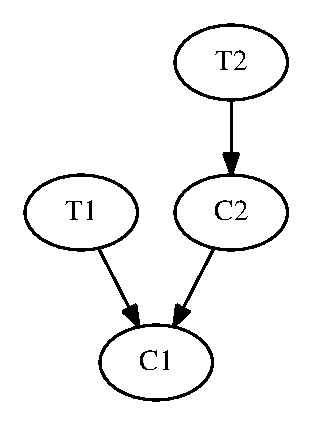
\includegraphics[scale=0.8]{dotGenerated/GraphExample.eps}}}
    \qquad
    \subfloat{{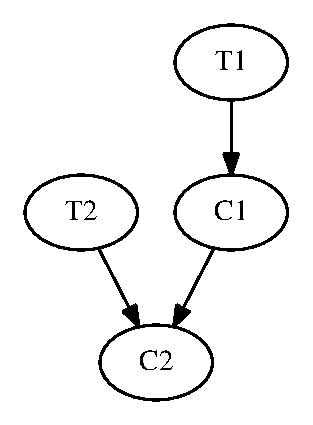
\includegraphics[scale=0.8]{dotGenerated/InvertedGraphExample.eps}}}
    \caption{To the left is a dependency graph and to the right is the corresponding inverted dependency graph. T1 and T2 are test cases and M1 and M2 are models}
    \label{fig:invertedGraph}
\end{figure}

\subsection{External functions}
The Modelica language allows the use of external functions that are not defined in a Modelica file. The external functions are often defined in a C-file.\cite{modelicamodelica}. In our dependency analysis we do not analyze the dependencies in external files. To handle this, and keep the test selection safe, if a non Modelica file is changed we assume that every Modelica class that depend on externals is affected.


\chapter[Evaluation]{Evaluation}
%TODO: Precision
%TODO: Hardware used
%TODO: Rework
%TODO: Dependency analysis time
In this chapter we are going to evaluate both the time savings and the precision of our dependency analysis. We have done measurements for HXL (the Heat Exchanger Library developed by Modelon) and MSL (Modelica Standard Library).
The time it takes to run the dependency analysis is not included in any of the graphs in this chapter.
To assess how much time our test selection can save we have run all the tests for each library several times to get the average time it takes to run each test. Then we have done the test selection for each Modelica file in the library and summed up the time for all tests that are selected when we say that file has changed. In Figure \ref{fig:hxlonefile} the total time to run the tests selected for each file in HXL is plotted. The files are on the x-axis and on the y-axis is the time for the selected tests, in percent of the time it takes to run all tests. The corresponding graph for MSL version 3.2.2 is in Figure \ref{fig:mslonefile}.

\begin{figure}[!htbp]
    \centering
    \makebox[\textwidth][c]{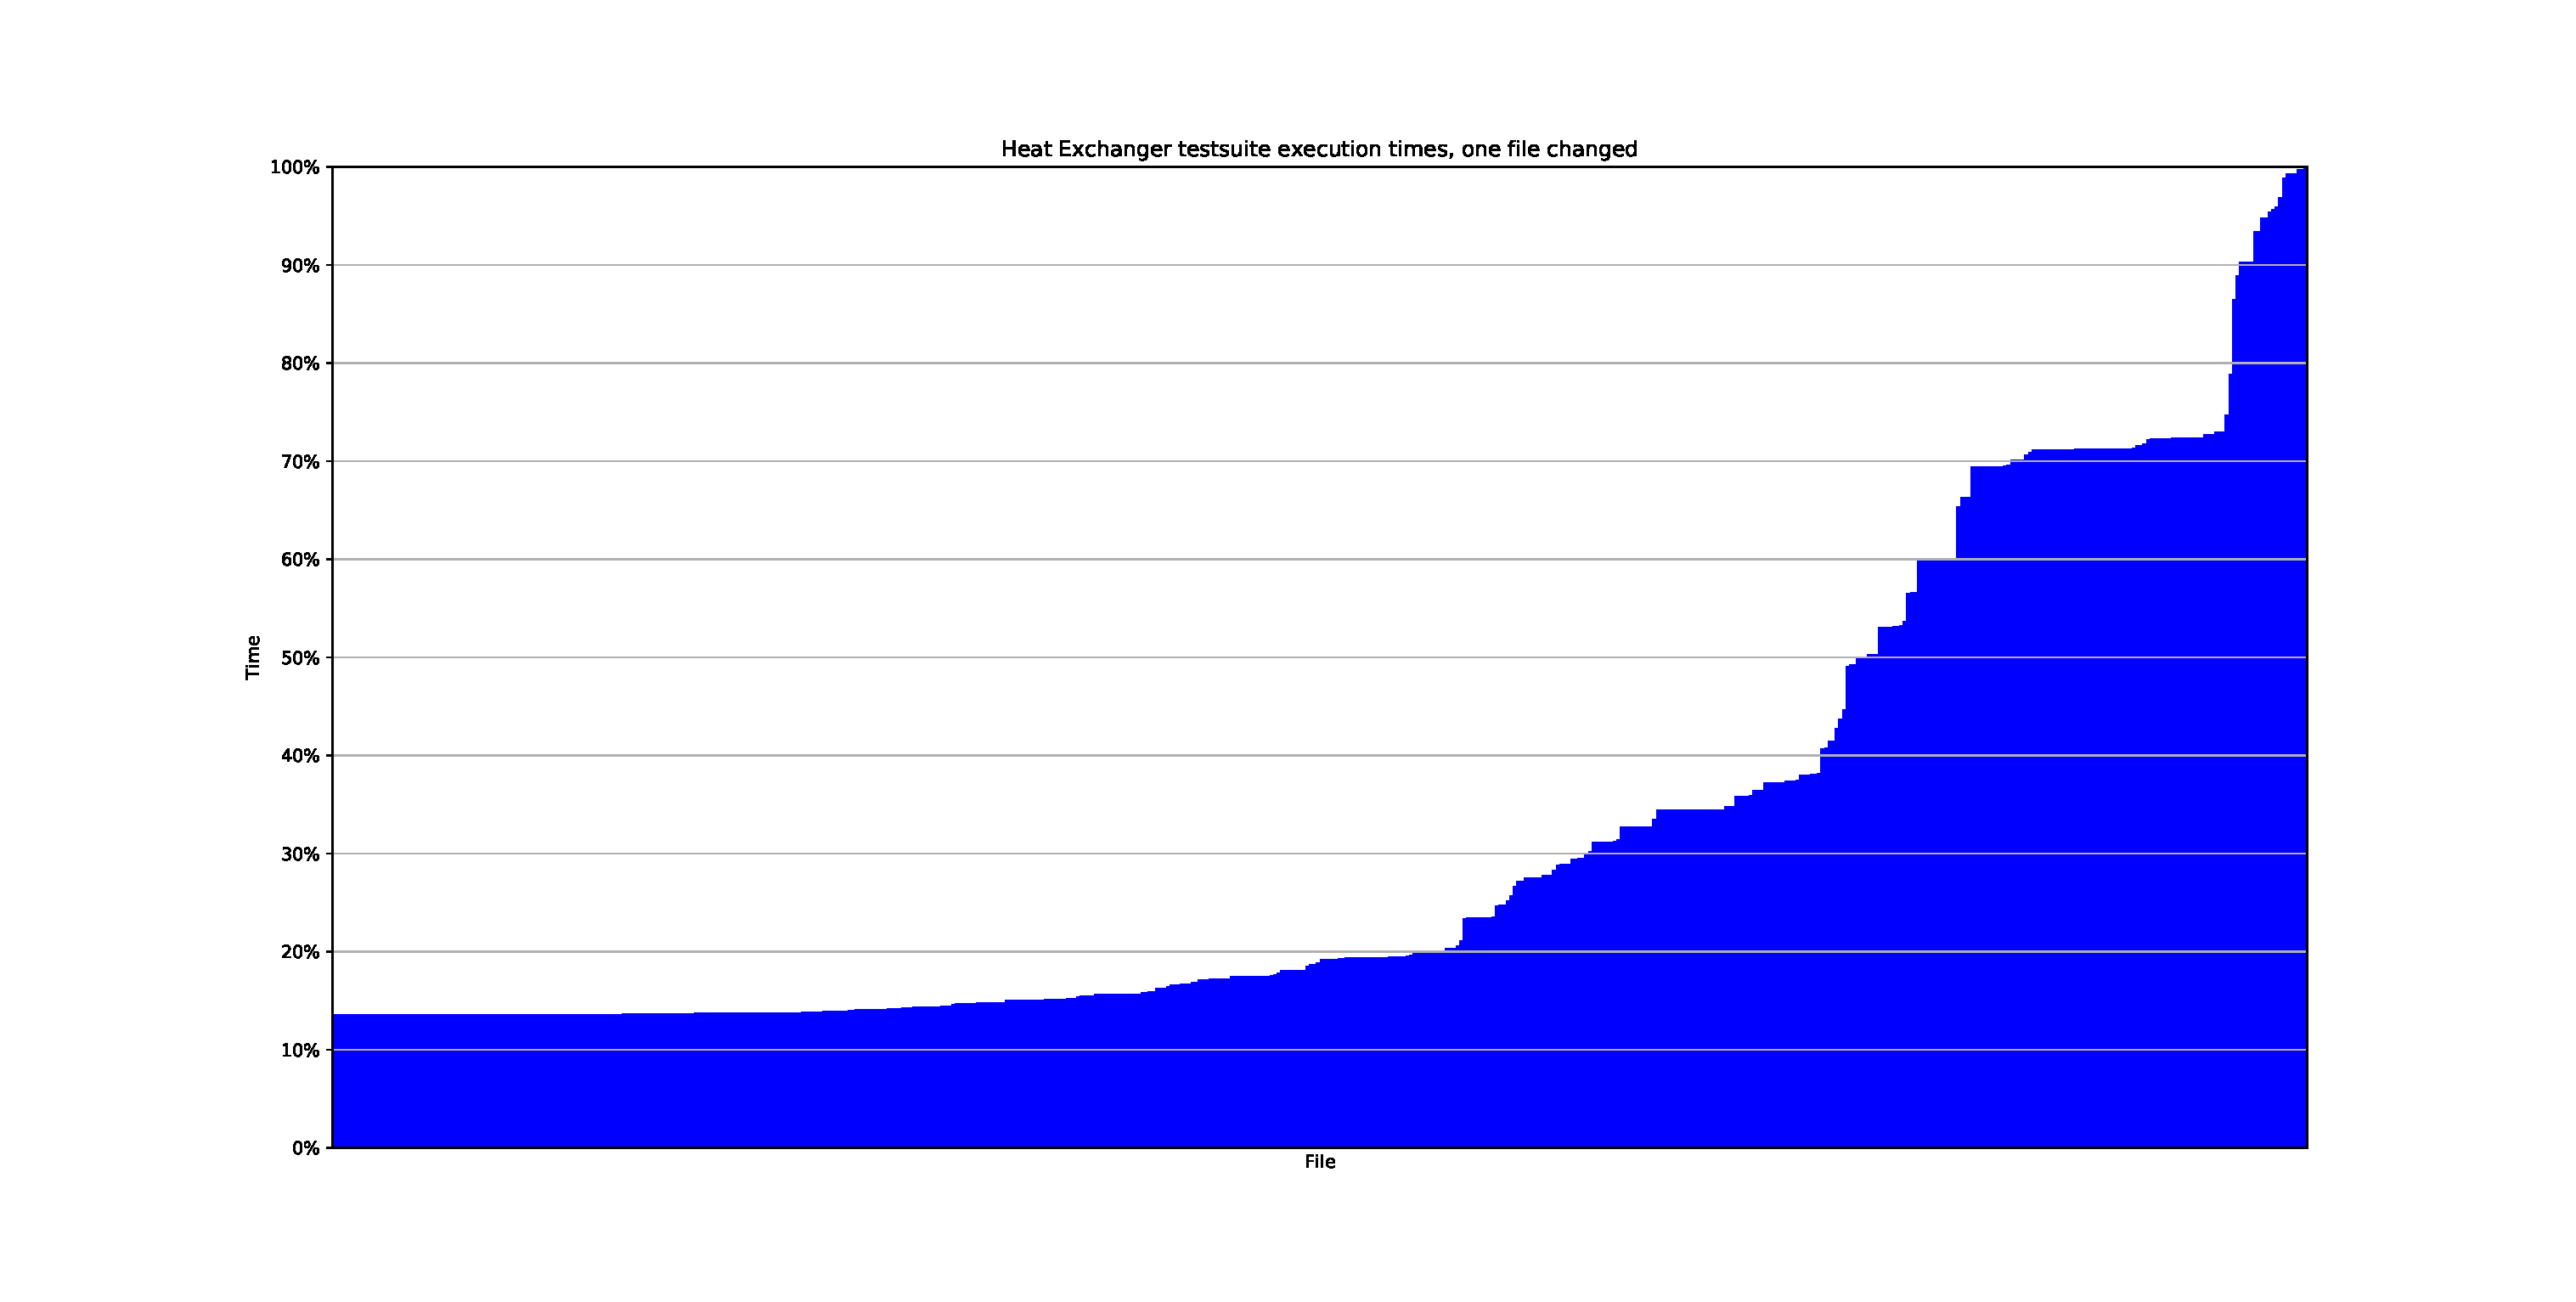
\includegraphics[width=1.5\textwidth]{Graphs/HXL_one_file.eps}}
    \caption{One file changed in HXL.}
    \label{fig:hxlonefile}
\end{figure}

\begin{figure}[!htbp]
    \centering
    \makebox[\textwidth][c]{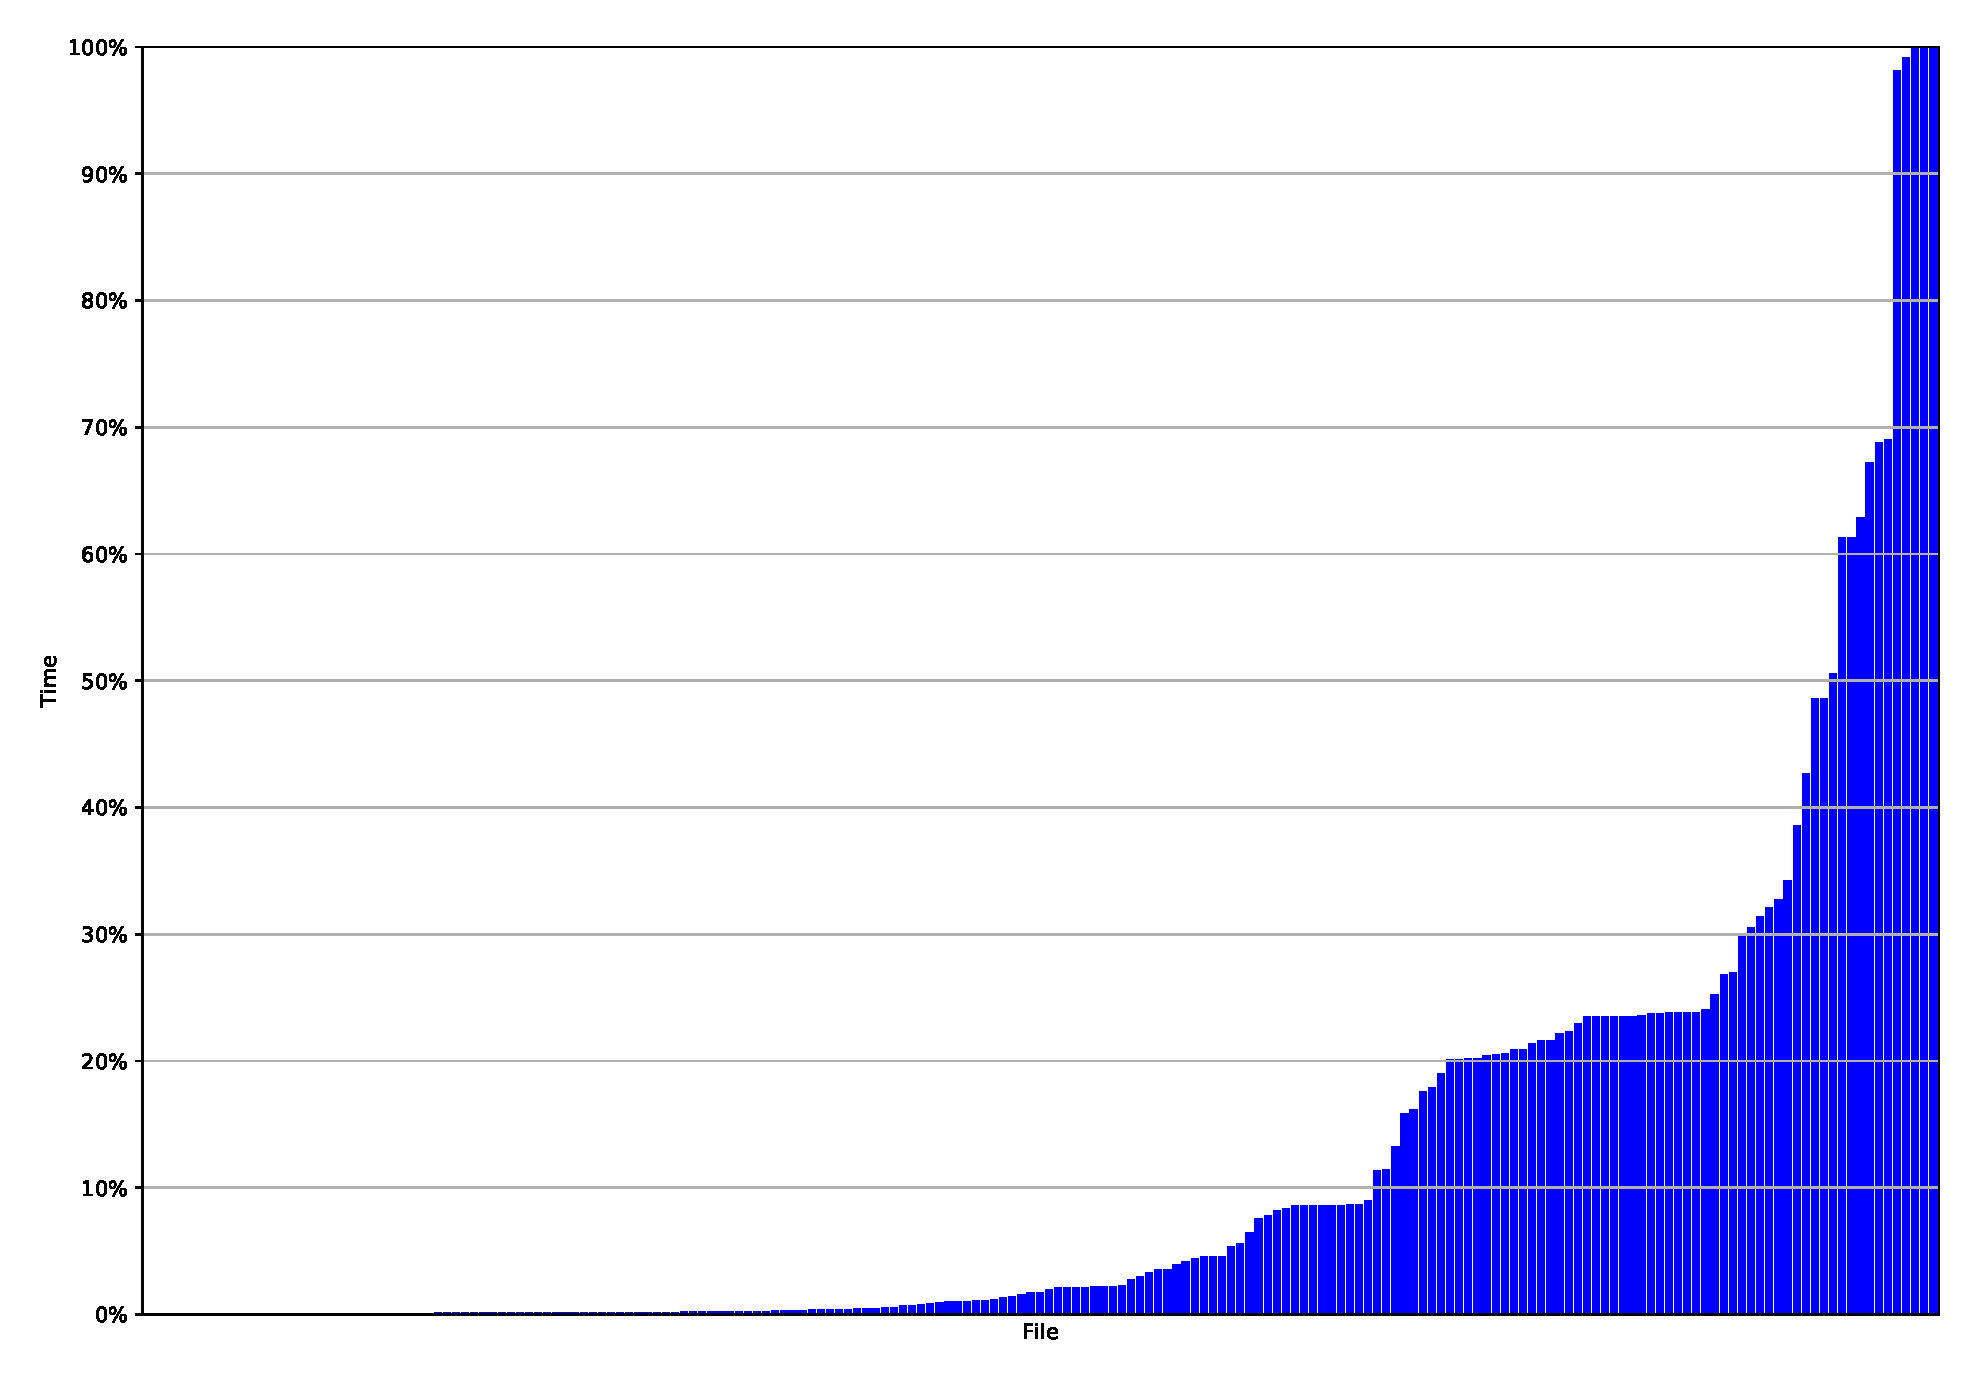
\includegraphics[width=1.5\textwidth]{Graphs/MSL_one_file.eps}}
    \caption{One file changed in MSL.}
    \label{fig:mslonefile}
\end{figure}

In Figure \ref{fig:mslhistory} we have used all the commits in the commit history for MSL until commit 2260. On the x-axis we have commits. On the y-axis we have the time for running all the tests that are selected when the test selection is done for the files that has changed in that commit. The time is here too plotted as the percent of the total time for running all tests. We have not run the dependency analysis for each version of the library in the commit history. We have only done the dependency analysis on the latest version and used that dependency graph for all versions. The average time saving for test executions in Figure \ref{fig:mslhistory} is 56\% per commit (time for running dependency analysis excluded).

\begin{figure}[!htbp]
    \centering
    \makebox[\textwidth][c]{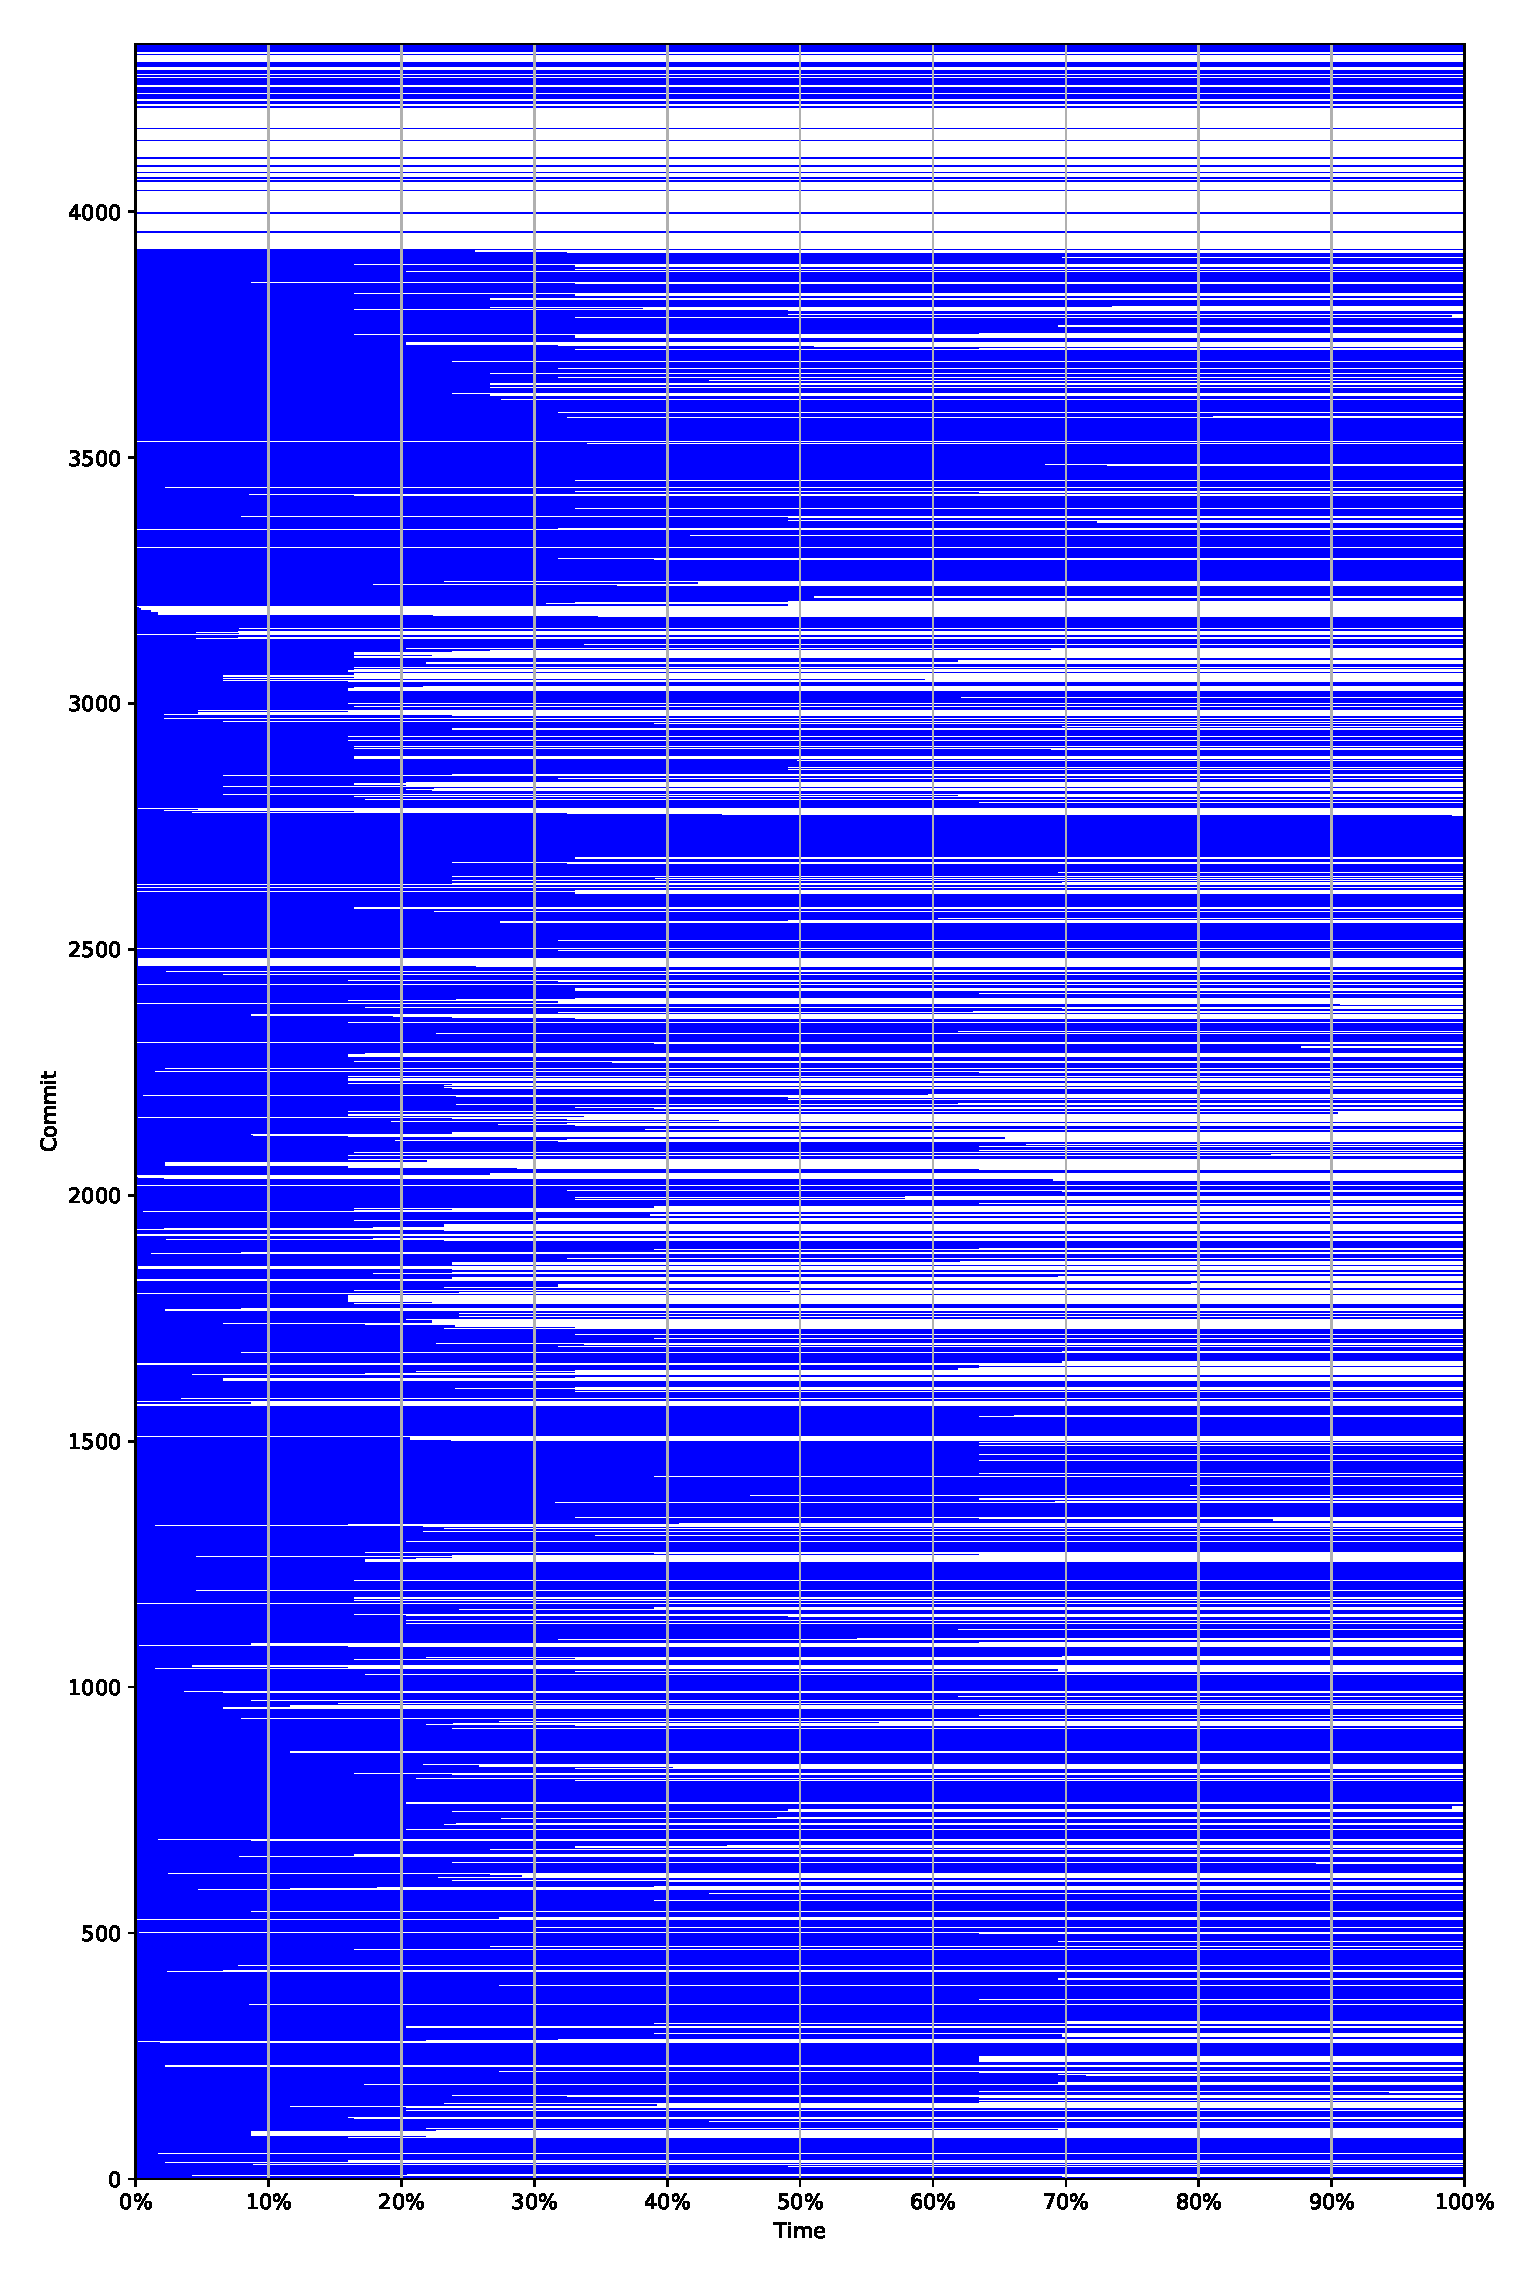
\includegraphics[width=1.5\textwidth]{Graphs/MSL_history_plot.eps}}
    \caption{History plot for MSL.}
    \label{fig:mslhistory}
\end{figure}
 
 Both Rule number 4, that we need due to limitations of the lookup in the source tree and the handling of files that is not Modelica files, lowers the precision of the test selection and creates extra overhead.

\chapter[Discussion]{Discussion}

\section{Validity}
Validating the test selection and is an important step to make sure the test selection actually is safe. 
However, is is not feasible to prove that the dependency analysis and our implementation is 100\% safe. Instead we have tried to prove that is not safe, but that can never prove that what we have built is safe. But, it will increase our confidence for the test selection. 

To do this we have a couple of approaches, firstly we hope to run our test selection parallel with the complete test suit on Modelon's build server to make sure all failed tests occurring have been caught by our test selection. This approach is inherently flawed since developers are actively trying to not commit code that breaks any tests. %%TODO: write some more?


Secondly we hope to do some mutation testing by introducing semi random errors in a library and then run all tests not in the test selection. If any test fails we know that the test selection is not safe. Both these approaches are basically the same except mutation testing is probably more effective since we can guarantee that there is problems in the code base. However, depending on the test coverage, every test could still pass.


\section{Granularity}
A dependency analysis can be performed with different granularities. Our dependency analysis handles classes and is sometimes converted to a more coarse analysis handling files. Generally a more coarse analysis will have lower precision since classes in the same file will be considered having the same dependencies. On the other hand moving to a more granular analysis can be costly ~\cite{DBLP:conf/sigsoft/LegunsenHSLZM16}, both in running time, complexity and size. A more granular analysis could for example handle dependencies between lines of code instead classes. This would have to be weighted against the precision gained.

We chose class granularity because is was easy to implement. Initially we wanted to perform the analysis at file level but when we started implementing it it was natural to go to class level since all the class level dependencies had to be resolved anyway to find the corresponding files. The results shows significant saving and therefor it is not motivated to increase the precision at the cost of analysis complexity, development time and running time.

\section{Modelica patterns}
%%TODO: How to write good Modelica code for this test selection


\section{Related Work}
% Kan kanske flyttas till bakgrunden ev till test selection delen. Måste inte ligga så sent i rapporten
A master thesis similar to this one has previously been done at LTH. In the previously master thesis JastAdd was used to decrease the cost for testing of Android projects ~\cite{kampe2012dependroid}. There is research done on test selection. A method for safe RTS for Java has been developed before, that has many similarities with the method we are developing for Modelica. 

Studies have been conducted to investigate at which granularity dependency analysis pays off the most and how much precision it can have without getting to expensive ~\cite{DBLP:conf/sigsoft/LegunsenHSLZM16}. It has also been done work in other techniques to achieve shorter time for testing, including dynamic test selection.

Safe regression test selection has been developed for Java at LTH \cite{DBLP:conf/pppj/OqvistHM16}. In this work the dependency graph i stored and updated when it changes unlike our solution for Modelica, where we compute the dependency graph each time. There is two main differences between Java and Modelica interesting for test selection. Modelica regression tests takes usually much longer time to run than Java regression tests. The longest time it takes to run all tests for a Java project used in the evaluation in \cite{DBLP:conf/pppj/OqvistHM16} is less than 20 seconds (on a 4-core 3.6GHz Intel i7-3820 CPU, with 64 GiB RAM, running Linux Mint 17.0). For the Modelica Standard Library it takes more than 2 hours to run all tests. In Modelica it is possible to use classes in another package without using imports, that is not possible in Java.
%TODO: Write somthing about the hardware we used
%TODO: Write about size of the Java project and MSL?

\chapter[Conclusion]{Conclusion}

%TODO: Write
%TODO: Significat time savings
%TODO: JModelica is not perfectly suited for this

\section{Future work}
\makebibliography{thebib}

%\begin{appendices}
%\chapter{About This Document}
%\end{appendices}


\end{document}